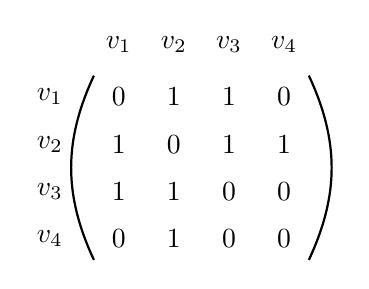
\begin{tikzpicture}[baseline=(current bounding box.center), x=0.7cm, y=0.6cm]
  % Matriz de adyacencia de G_{13}, llenada progresivamente
  % Etiquetas de filas y columnas
  \foreach \k in {1,...,4} {
    \node at (\k,0.1) {$v_{\k}$};
    \node at (-0.25,-\k) {$v_{\k}$};
  }
  % Paréntesis
  \draw[thick] (0.55,-0.55) to[bend right=25] (0.55,-4.45);
  \draw[thick] (4.45,-0.55) to[bend left=25] (4.45,-4.45);
  % Entradas: {fila/columna/valor/diapositiva de aparición}
  \foreach \fil/\col/\val/\dia in {1/1/0/2, 1/2/1/3, 1/3/1/4, 1/4/0/5,
                           2/1/1/6, 2/2/0/7, 2/3/1/7, 2/4/1/7,
                           3/1/1/7, 3/2/1/7, 3/3/0/7, 3/4/0/7,
                           4/1/0/7, 4/2/1/7, 4/3/0/7, 4/4/0/7}
    \node<\dia-> at (\col,-\fil) {$\val$};
\end{tikzpicture}
